\chapter{Estado del arte}

En esta sección se analiza el estado de la investigación en los algoritmos de optimización bio-inspirados, con respecto a 
librerías o \emph{frameworks} disponibles, además de la investigación y el estado actual de las metaheurísticas. Se van a analizar
estos conceptos, ya que se pretende establecer el punto de partida sobre el que se base este trabajo.

\section{Algoritmos bio-inspirados}

Hay una evidencia clara en la creciente popularidad ganada por los algoritmos bio-inspirados en las últimas 2 décadas. Según D. Molina \cite{Molina2020ComprehensiveTO} esto se
debe a la capacidad que tienen este tipo de algoritmos para aprender, adaptarse y dar buenas soluciones a problemas complejos que de otra manera se hubieran quedado sin
resolver. Estos algoritmos imitan procesos biológicos o estructuras presentes en la naturaleza, y se aplican para resolver problemas de optimización. Por ejemplo, 
la \textbf{Optimización por Nube de Partículas} o PSO (\textit{Particle Swarm Optimization}) que imita el comportamiento de las partículas en la naturaleza, o 
el \textbf{Algoritmo colonia de abejas} basado en el comportamiento de los enjambres de abejas para encontrar la miel. 

Esta gran cantidad de metaheurísticas basadas en metáforas ha sido criticada por algunos autores como K. Sörensen\cite{metaphor_exposed}, 
que considera que esta línea de investigación amenaza con separar el ámbito de las metaheurísticas del rigor científico. 
En su paper \emph{Metaheuristics - the metaphor exposed} concluye que las metaheurísticas basadas en nuevas metáforas deberían 
evitarse si no pueden demostrar una nueva aportación al campo. Además este tipo de algoritmos suelen usar terminología inspirada por el dominio, 
lo que conduce a nuevos términos que describen conceptos que ya estaban establecidos \cite{mitigating_metaphors}, lo que a su vez hace que sea difícil 
entender cómo funcionan estos algoritmos y la relación que tienen con otras metaheurísticas. 

La falta de universalidad que sobrepasa las metaheurísticas para cualquier tipo de problema de optimización proviene
del conocido teorema de optimización \emph{``No Free Lunch''}, que demuestra que si un algoritmo se comporta bien en cierto tipo de 
problemas entonces pagará por eso con un peor rendimiento en el resto de problemas \cite{585893}. Autores como 
Swan \cite{metaheuristics} establecen que para que la investigación en el campo de las metaheurísticas evite la fragmentación y la falta de reproductibilidad, se 
necesita una infraestructura científica y computacional fuerte, donde diferentes enfoques puedan ser desarrollados, analizados y comparados. 

El algoritmo presentado en este trabajo evita caer en el uso de metáforas para explicar su comportamiento. Se inspira en ellas para crear una estructura de datos que ayude 
a mantener la diversidad a lo largo de toda la ejecución. Además, toda la terminología y conceptos usados a lo largo del proyecto son los acuñados hasta ahora en este campo.

\section{Implementación}

Otro de los problemas presentes en el campo de las metaheurísticas es la falta de reutilización \cite{metaheuristics}. Se trata de una falta en cuanto a implementación, ya que hay una
tendencia a re-implementar los algoritmos desde 0, impidiendo la reproducibilidad. El progreso científico en cualquier disciplina requiere de la habilidad de construir sobre lo que
otros ya han hecho para poder llegar más lejos. Por ello el algoritmo desarrollado ha sido publicado en un registro de paquetes, además se ha hecho de manera que se pueda usar para 
cualquier de problema de optimización. 

Normalmente en este campo, el código usado para realizar los experimentos descritos en la literatura no se suele describir. En los
pocos casos en los que se adjunta código suele ser código sucio, o usa lenguajes privativos y los resultados se hacen en repositorios cerrados. 
Mientras que la forma de implementar el código no es una prioridad en la programación científica, 
en campos como el desarrollo web, seguir ciertos estándares como arquitectura limpia \cite{cleanArquitecture2017} y la 
limpieza del código \cite{cleanCode2008}, así como el desarrollo basado en tests, es algo básico.

\section{Lenguajes de programación en el ámbito científico}

Hay un mito muy extendido en programación científica que afirma que los lenguajes compilados como C++ o Java son siempre más rápidos que los lenguajes interpretados como Python o 
JavaScript. Atendiendo a este mito, los lenguajes más usados en el desarrollo metaheurísticas son: Matlab, C++, Python o Java \cite{languages}. Siendo Python el más 
utilizado debido a la cantidad de librerías disponibles, con algoritmos genéticos listos para usar, o la facilidad para extraer gráficas de los resultados. En general, a 
la hora de lanzarte a programar un proyecto relacionado con \emph{Aprendizaje Automático} o \emph{Inteligencia Artificial}, es el primer lenguaje que se viene a la cabeza. 

Elegir el lenguaje de programación con el que se va a desarrollar el proyecto es una decisión importante. Sin embargo atendiendo al trabajo de J.J. Merelo \cite{fast_lunch}, aunque
la velocidad parezca un criterio importante a tener en cuenta, el \emph{paper} afirma que, en la misma línea del teorema \emph{There is no free lunch}, se cumple el teorema
\emph{There is no fast lunch}. Este último teorema establece, que aunque algunos lenguajes podrían ser más rápidos para ciertos tamaños de problemas y 
funciones de fitness, en general el lenguaje más rápido dependerá de esas dos cosas.

A pesar del teorema mencionado en el párrafo anterior, para el desarrollo se descarta el uso de Python; si bien tiene una gran cantidad de bibliotecas disponibles con algoritmos 
genéticos ya desarrollados y una extensa comunidad, en la primera implementación de este algoritmo se usó este lenguaje \cite{merelo_molina_2021} y las prestaciones no fueron muy altas. 
El algoritmo tardaba del orden de horas en terminar, lo que complicaba mucho el análisis del mismo. Gmys \cite{comparative_study} compara varios lenguajes en términos de rendimiento, 
escalabilidad y productividad. En su trabajo menciona lenguajes como \emph{Julia} o \emph{Chapel}. El objetivo de \emph{Julia} es acoplar la brecha de rendimiento en la programación, 
ofreciendo a los programadores científicos un lenguaje para el prototipado rápido y la computación de altas prestaciones. Sin embargo, al ser un lenguaje joven, ha habido bastantes
cambios desde las primeras versiones. Así, la mayoría de la información en foros que está disponible, está desactualizada, lo que lo hace un lenguaje difícil para aprender.
No obstante, su popularidad está aumentando; una de las principales razones es su unión en 2017 al ``Club Petaflop``, que confirma el buen rendimiento que puede llegar a ofrecer.  

\section{\textit{Frameworks} para algoritmos genéticos}

Hay un alto número de \emph{framworks} disponibles para el desarrollo de algoritmos genéticos. En el caso de Python los más populares son:

\begin{enumerate}
    \item \emph{DEAP} \cite{deap}: permite desarrollar algoritmos genéticos (entre muchas utilidades más) en Python. Se define como un \emph{framework}
    de computación evolutica para el prototipado y prueba rápida de ideas.
    \item \emph{PyGAD} \cite{pygad}: es una librería de código abierto para la construcción de algoritmos genéticos y para la optimización de algoritmos
    de aprendizaje automático. Contiene operadores de evolución ya definidos entre los que hay que elegir; no se puede definir uno propio.
\end{enumerate}

Las librerías mencionadas se adaptan muy bien al problema a afrontar, pero como ya se ha mencionado, no se va a usar Python para el desarrollo por su baja
velocidad. Para el lenguaje \emph{Chapel} no se ha encontrado ninguna biblioteca popular que sea importante mencionar. Actualmente hay varios
\emph{frameworks} disponibles en \emph{Julia} para programación de algoritmos evolutivos. Se va a mencionar brevemente su uso, además de por qué no
se adaptan a las necesidades de este TFG.

\begin{enumerate}
    \item \emph{Metaheuristics.jl} \cite{metaheuristics_jl}: Este paquete implementa metaheurísticas para la optimización global. Su objetivo es proporcionar metaheurísticas
    fáciles y rápidas de usar para la optimización global numérica. El comportamiento es muy parecido al que queremos desarrollar, contiene una función \emph{optimize}
    a la que se le pasa la función fitness, el rango, y opciones como el máximo número de llamadas a la función de fitness. Es una opción muy interesante, el problema es que las
    metaheurísticas están ya predefinidas.
    \item \emph{GeneticAlgorithms.jl} \cite{GeneticAlgorithms_jl}: es un \emph{framework} ligero que simplifica el proceso de creación de algoritmos genéticos y su ejecución en
    paralelo. Podría haber sido fácilmente usado para este trabajo, ya que tú misma puedes definir los operadores y la función que quieres que use el algoritmo. El problema es
    que los argumentos que se le pueden pasar a estos operadores vienen predefinidos, por lo que no puedes usar \emph{dispatch} múltiple pare diferenciar entre los individuos de 
    la población.
    \item \emph{Darwin.jl} \cite{darwin_jl}: está basado en \emph{GeneticAlgorithms.jl}, por lo que presenta el mismo problema que el anterior.
    \item \emph{Evolutionary.jl} \cite{evolutionary_jl}: el objetivo es proveer una biblioteca para optimización evolutiva. Proporciona mucha flexibilidad a la hora configurar los parámetros
    de entrada. El problema que presenta es que, a pesar de ofrecer varios tipos de operadores genéticos, no puedes usar unos personalizados.
    \item \emph{JuMP.jl} \cite{DunningHuchetteLubin2017}: es un lenguaje para el modelado de problemas cuyo dominio sea la optimización matemática. Incluye muchas opciones para la personalización,
    además de muchos tipos de modelos para diferentes tipos de problemas. Pese a lo completo que es este \emph{framework}, no incluye soporte para algoritmos genéticos.
\end{enumerate}

\subsection{Comparación con \emph{GeneticAlgorithms.jl}}

Para establecer el estado del arte en velocidad y prestaciones del algoritmo y el lenguaje, vamos a probar
el \emph{framework} \emph{GeneticAlgorithms.jl}. Se ha elegido esta librería porque te permite definir los operadores que se van a usar, además es la más sencilla de aprender,
ya que está orientada únicamente al desarrollo de algoritmos genéticos. Se va a usar con los operadores implementados en el ejemplo definido por el autor. Los individuos 
irán definidos por el cromosoma y el valor de la función del fitness. Para ello, previamente hay que instalarlo.

El repositorio del proyecto lleva desde 2017 sin actualizarse, esto no debería ser un problema, pero como menciona Gmys \cite{comparative_study}
en su trabajo, Julia es un lenguaje joven que ha tenido cambios grandes. En este repositorio encontramos uno de esos casos. Al intentar compilarlo la primera vez dio error, porque contiene
palabras propias del lenguaje antiguas. Por ejemplo, antes para definir estructuras de datos se usaba la palabra \emph{type} y ahora se usa \emph{struct}. Como se trata de una de las pocas 
bibliotecas que hay para comparar la nuestra, y adicionalmente solo tiene un par de ficheros, se ha actualizado como parte de este TFG. Se ha creado un \emph{pull request} al repositorio del proyecto. 
Los operadores que se han definido son los que se encuentran en los ejemplos del proyecto. Se va a probar para un tamaño de población 100, y como función de Fitness: Rastrigin, 
que es la que se usará para los experimentos de nuestro algoritmo en secciones futuras. Se trata de una función multimodal, con $10^{D}$ óptimos locales, por lo que el algoritmo 
tiene muchas posibilidades de converger rápido. Se ha elegido para las exploraciones iniciales porque se encuentra en el punto medio de no ser tan fácil como la función de Esfera 
que está definida en un espacio continuo, pero tiene que mantener la diversidad para
no estancarse.

La librería devuelve la última población del algoritmo antes de parar, los valores de Fitness resultantes en la última generación se pueden ver en la Figura \ref{fig:genetic_algorithms_jl},
el resumen de la ejecución. "Estos valores nos servirán como línea base de comparación con nuestro algoritmo". No se puede evaluar bien el comportamiento de este \emph{framework} ya que 
la única información disponible para el análisis es el estado de la población en la última generación. Salvo por el problema de la sintaxis antigua y la falta de datos,
ha sido bastante fácil de usar, además permite mucha flexibilidad. Como elementos a destacar: Se pueden personalizar casi por completo todos los operadores. Otra

\begin{figure}[H]
	\centering	
	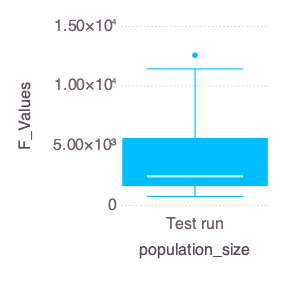
\includegraphics[scale=0.6]{../data/Plots/comparation.png}
	\caption{Ejecución para probar la librería \emph{GeneticAlgorithms.jl}. Se ha ejecutado para un tamaño de población de 100. Como función de fitness Rastrigin.}
    \label{fig:genetic_algorithms_jl}
\end{figure}

